We design \ModelName{} for agentic systems that operate over complete trajectories to produce: (i) comprehensive error detection across all steps and modules, and (ii) causal root-cause diagnosis with actionable feedback. The core principle is to identify the earliest critical decision whose correction would flip the trajectory from failure to success. This section describes our unified agent formulation, error taxonomy, and the two-stage debugging pipeline.

\begin{figure}[htbp]
    \centering
    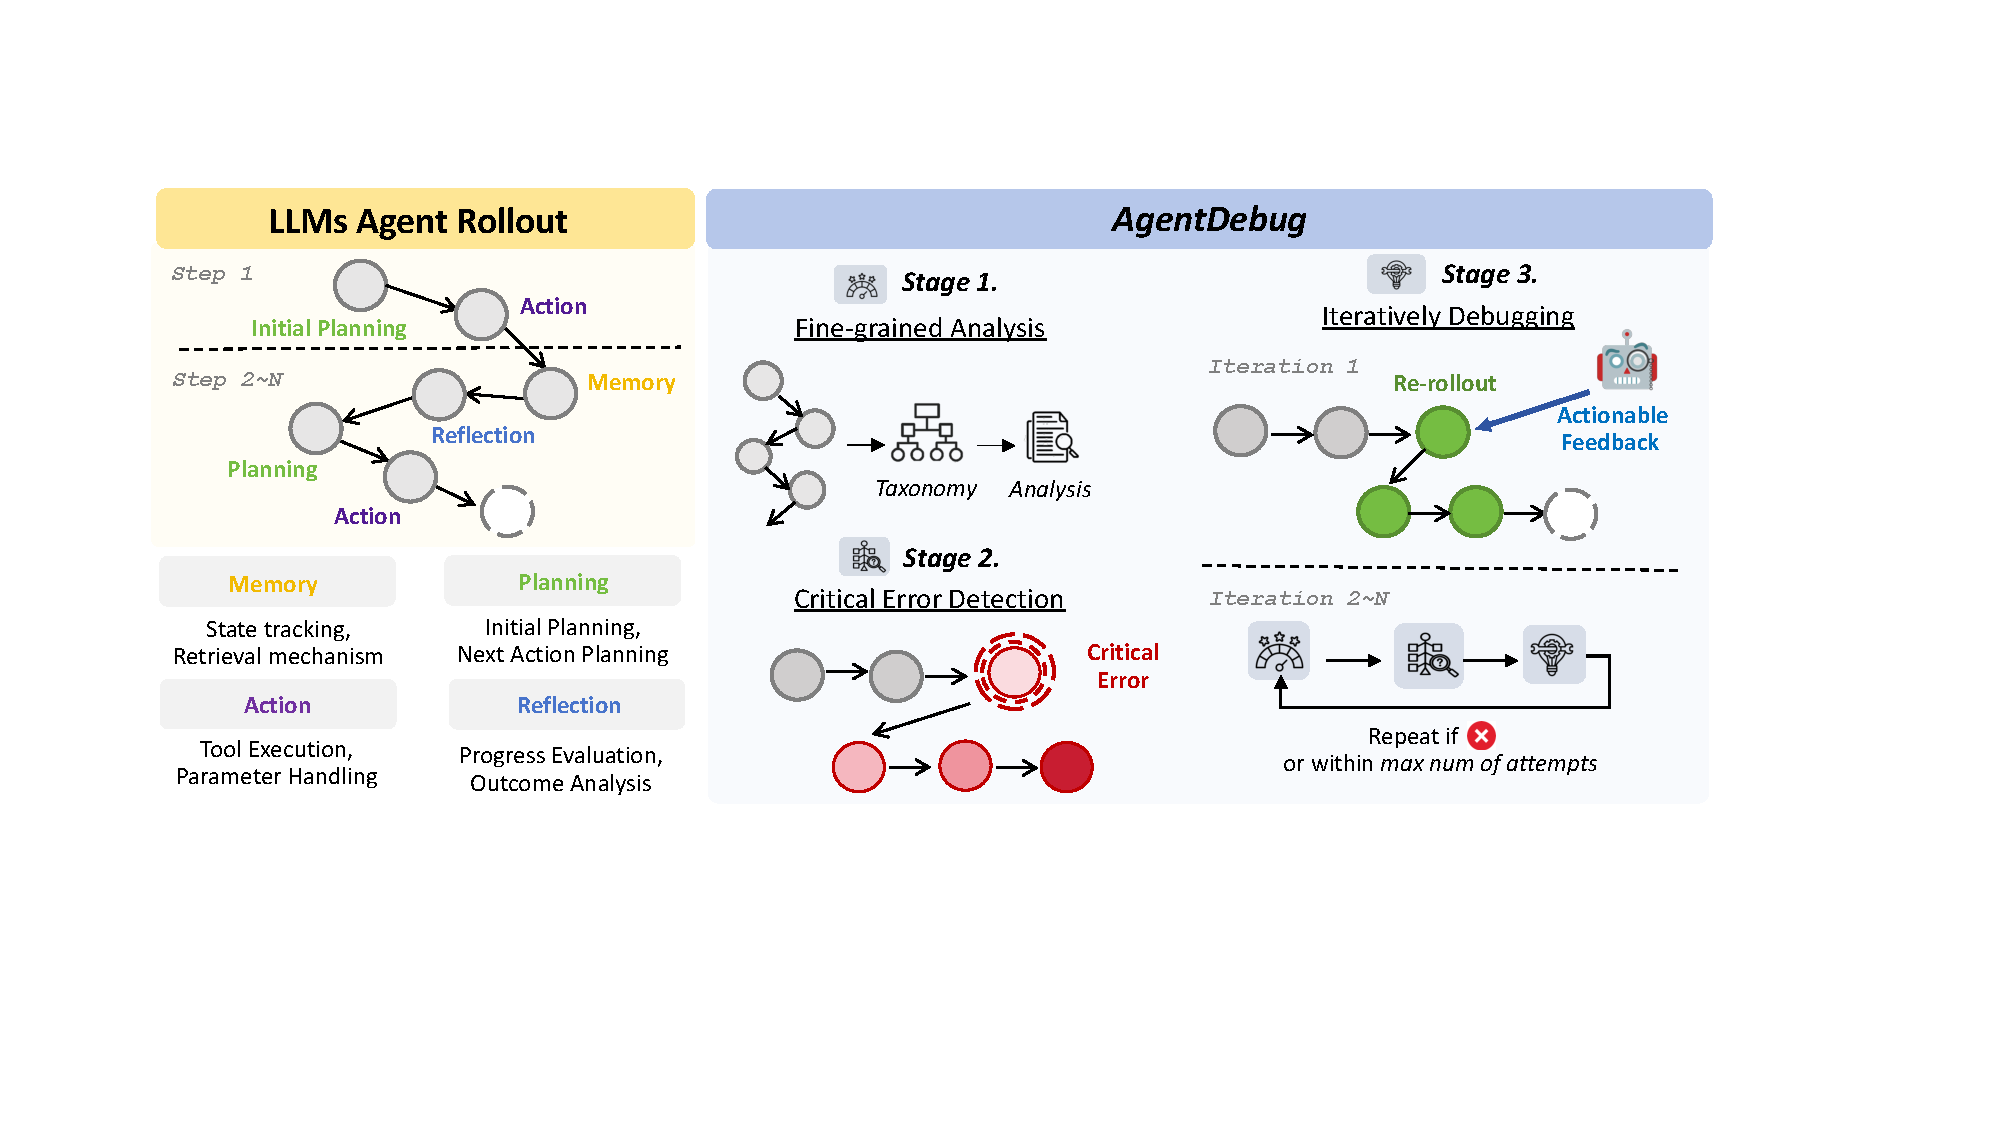
\includegraphics[width=1\linewidth]{figures/method.pdf}
    \caption{\textbf{Overview of \ModelName{}.} (Left) Core modules—\emph{Planning}, \emph{Action}, \emph{Memory}, \emph{Reflection}—operate across varied environments. (Center) Unified rollout: Step~1 global plan, then plan$\rightarrow$act$\rightarrow$observe with memory/reflection updates. (Bottom) Failures are debugged into successes via actionable feedback, yielding paired traces. (Right) Training: Stage~1 step-level \emph{Error Detector}; Stage~2 global \emph{Root-Cause Analyzer} that pinpoints the earliest causal error and prescribes a fix.}

    \label{fig:method}
\end{figure}


\subsection{Error Detector Design}

Our debugging framework operates in two complementary stages: comprehensive error scanning followed by causal root-cause analysis. This design balances exhaustive detection with targeted intervention.

\paragraph{Stage 1: Comprehensive Error Detection}

Stage 1 functions as an error scanner that identifies all potential failures across the trajectory. For each step $t$, we detect the presence of error types from our taxonomy using a multi-label classifier:
$$p(\mathbf{y}_t \mid \tau_{\leq t}) = g_\theta(\text{Context}(s_{\leq t}, a_t, o_t))$$
where $\mathbf{y}_t \in \{0,1\}^K$ indicates $K$ error types. We implement $g_\theta$ as an instruction-tuned LLM (Qwen-8B/14B) prompted with the AET schema and few-shot examples. The model outputs structured predictions $(t, \mathcal{E}_t, \text{rationale}_t)$ containing detected errors and supporting evidence.

\paragraph{Stage 2: Causal Root-Cause Analysis}

While Stage 1 identifies where errors occur, Stage 2 determines which error caused the trajectory failure through causal reasoning. This distinction is crucial—many detected errors are symptoms rather than root causes.

\paragraph{Causal Criterion.} We identify the root cause as the earliest step whose correction would likely lead to task success. Formally, let $U(\tau) \in \{0,1\}$ indicate task success and $\mathsf{fix}_t(\tau)$ denote a minimal edit correcting step $t$'s error. We select:
$$t^* = \arg\min_t \; t \quad \text{s.t.} \quad \mathbb{P}[U(\mathsf{fix}_t(\tau)) = 1] \geq \gamma$$

This identifies the earliest intervention point with sufficient impact on the outcome.

\paragraph{Implementation.} Computing exact counterfactual probabilities is intractable. We implement root-cause analysis using GPT-4.1 as an LLM judge that performs causal reasoning over the complete trajectory. The judge takes as input the Stage 1 error detections $\{\mathcal{E}_t\}_{t=1}^T$ and the full trajectory $\tau$, then outputs a structured diagnosis:
$$\text{RootCause}(\tau, \{\mathcal{E}_t\}) \rightarrow \langle t^*, \text{error\_type}, \text{reasoning}, \text{feedback} \rangle$$

where $t^*$ identifies the critical step, $\text{error\_type} \in \text{AET}$ specifies the root-cause error category, $\text{reasoning}$ provides the causal chain analysis, and $\text{feedback}$ contains actionable correction instructions.

To optimize the LLM judge's accuracy, we conducted iterative refinement using our human-annotated validation set from AgentErrorBench. Through multiple rounds of prompt engineering and few-shot example curation, we improved the judge's performance in identifying true root causes versus superficial symptoms. The refinement process involved:
\begin{align}
\text{Judge}^{(k+1)} = \text{Refine}(\text{Judge}^{(k)}, \mathcal{V}_{\text{human}})
\end{align}

where each iteration incorporated failure cases from the previous round as additional few-shot examples and adjusted the causal reasoning instructions based on disagreements with human annotations. After five refinement iterations, our GPT-4.1 judge achieved 87\% accuracy in root-cause identification and 91\% agreement with human annotators on critical step selection, validated on a held-out test set of 100 expert-labeled trajectories.


\subsection{Inference}

Once the root cause $t^*$ is identified, \ModelName{} generates structured actionable feedback $\mathcal{F}_{t^*}$ containing four key components:
\begin{align}
\mathcal{F}_{t^*} = \langle \text{step}_{t^*}, \text{error\_type} \in \text{AET}, \text{correction}, \text{rationale} \rangle
\end{align}

where $\text{step}_{t^*}$ identifies the critical failure point, $\text{error\_type}$ specifies the categorized failure from our taxonomy, $\text{correction}$ provides a concrete fix (e.g., "Replace API call `search(query='hotels')` with `search(query='hotels', location='Paris')`"), and $\text{rationale}$ explains the causal chain (e.g., "The missing location parameter caused all subsequent hotel bookings to fail as they targeted wrong cities"). This feedback is designed to be interpretable and actionable, enabling agents to understand not just what went wrong, but why it matters for task completion.

The targeted intervention proceeds through localized re-rollout:
\begin{align}
\tau_{\text{new}} = \langle \tau_{<t^*}, \text{apply}(\mathcal{F}_{t^*}), \text{rollout}(s_{t^*}', \pi_{\text{corrected}}) \rangle
\end{align}

\paragraph{Iterative Debugging with Retry Budget.}
Recognizing that complex tasks may require multiple rounds of debugging, \ModelName{} supports iterative refinement with a retry budget $N$. The complete debugging loop operates as follows:
\begin{align}
\text{for } i = 1 \text{ to } N: \quad \tau^{(i)} = \begin{cases}
\tau^{(i-1)} & \text{if } U(\tau^{(i-1)}) = 1 \text{ (success)} \\
\text{Debug}(\tau^{(i-1)}) \rightarrow \tau_{\text{new}} & \text{if } U(\tau^{(i-1)}) = 0 \text{ (failure)}
\end{cases}
\end{align}

At each iteration, if the current trajectory fails, our error detector performs the two-stage analysis (comprehensive detection followed by root-cause identification), generates targeted feedback, and executes a localized re-rollout from the identified critical step. This process continues until either: (1) the task succeeds, or (2) the retry budget $N$ is exhausted. In practice, we find that $N=3$ strikes an effective balance between performance gains and computational cost, with most recoverable failures being resolved within 2 iterations. This iterative capability allows \ModelName{} to handle cascading failures where fixing one root cause may reveal another underlying issue, ultimately achieving up to 23\% improvement in task success rates compared to single-attempt baselines.


\paragraph{Iterative Debugging Pipeline.}
The complete \textbf{AgentDebug} pipeline iteratively applies the detect-diagnose-fix cycle up to $N$ times within a test-time compute budget. At each iteration $k$:
\begin{align}
\tau^{(k+1)} = \text{AgentDebug}(\tau^{(k)}) = \begin{cases}
\tau^{(k)} & \text{if } U(\tau^{(k)}) = 1 \\
\text{Rerun}(\tau^{(k)}, \mathcal{F}_{t^*}^{(k)}) & \text{otherwise}
\end{cases}
\end{align}
